	\chapter{Działanie programu}
	Program rozpoczyna swoje działanie wygładzaniem chmury punktów. Jest to krok który ułatwia wykonanie dalszych algorytmów. Na rysunku \ref{fig:smoothcloudbefore} przedstawiono przybliżony widok chmury punktów przed wygładzaniem. Rysunek \ref{fig:smoothcloudafter} przedstwia przybliżenie na część punktów po wygładzeniu całej chmury.\\
	\begin{figure}[!htb]% ładne wstawienie obrazków obok siebie
		\begin{minipage}{0.48\textwidth}
			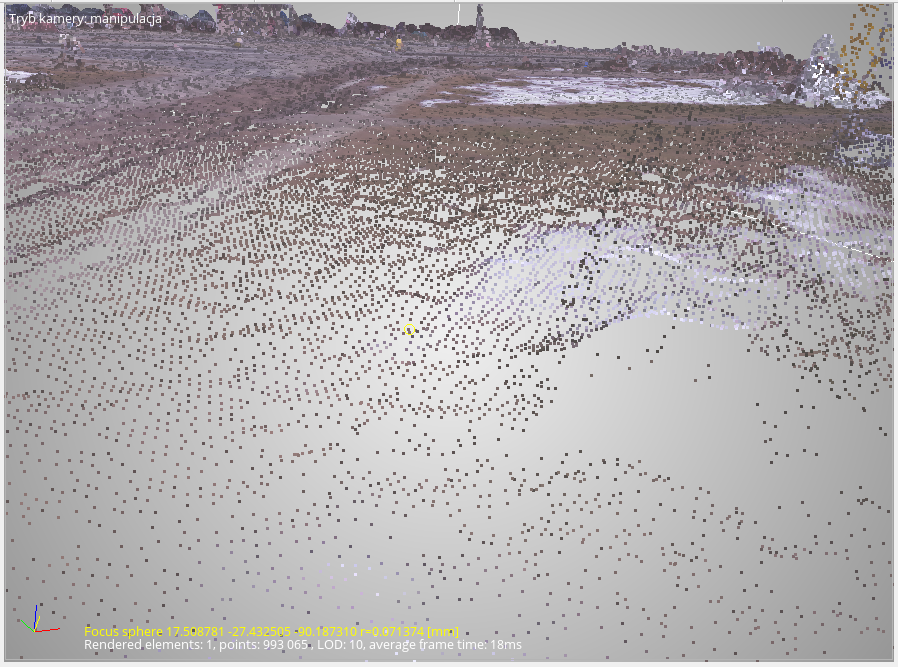
\includegraphics[width=\linewidth]{smoothing_cloud_before.png}
			\caption{Chmura punktów przed wygładzeniem}
			\label{fig:smoothcloudbefore}
		\end{minipage}\hfill
		\begin{minipage}{0.48\textwidth}
			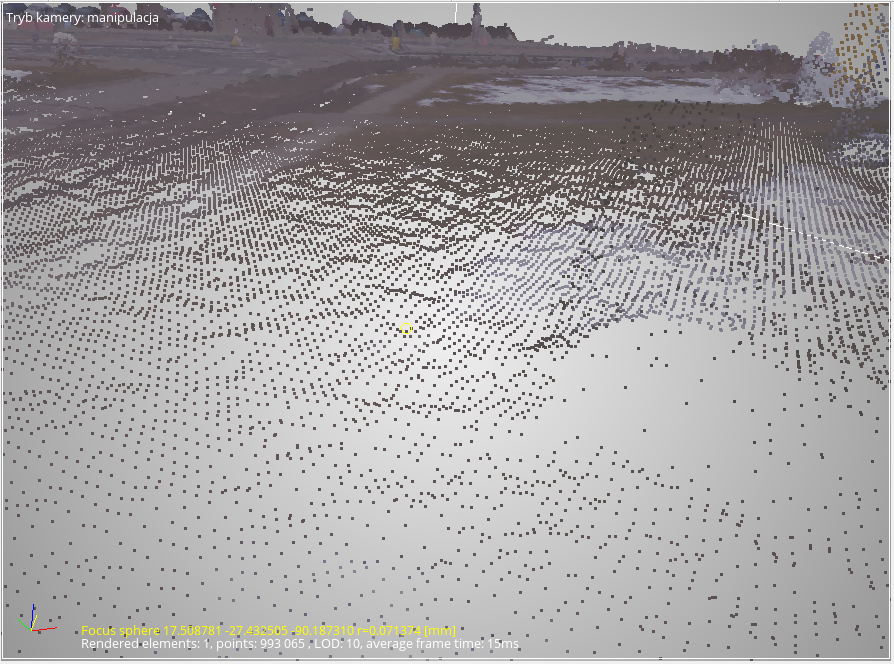
\includegraphics[width=\linewidth]{smoothing_cloud_after.png}
			\caption{Chmura punktów po wygładzeniu}
			\label{fig:smoothcloudafter}
		\end{minipage}\hfill
	\end{figure}

	Kolejnym krokiem koniecznym do segmentacji jest obliczenie wektorów normalnych dla każdego punktu. Dzieje się to przy użyciu najlepiej dopasowanej płaszczyzny do rozważanego punktu oraz jego sąsiedztwa wyrażonego przez ilość sąsiadów.\\
	\newpage
	\begin{figure}[h!]
	\centering
	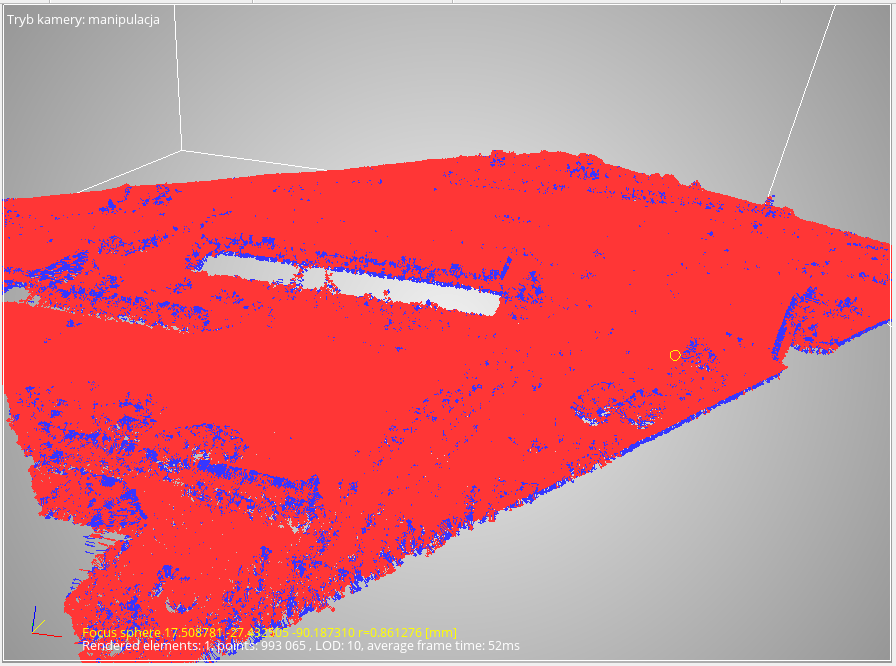
\includegraphics[width=0.85\textwidth]{normal_vectors.png}
	\caption{Wektory normalne}
	\label{fig:normalvecs}
	\end{figure}
	
	Na podstawie obliczonych wektorów normalnych, liczone są kąty między nimi a osią Z. Zapisywane są one do warstwy Horizontal Angles.\\
	\begin{figure}[h!]
	\centering
	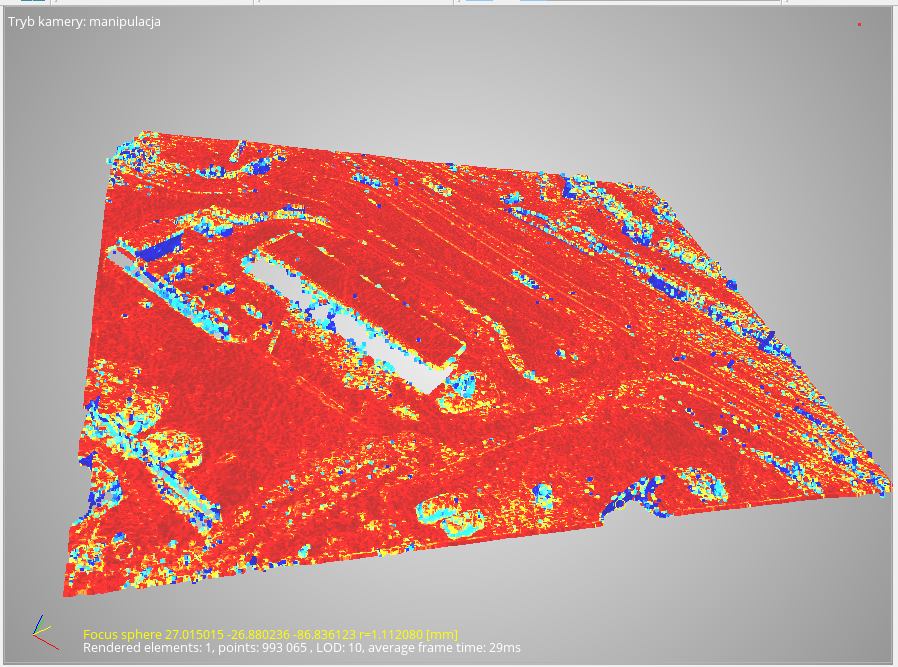
\includegraphics[width=0.85\textwidth]{horizontal_angles.png}
	\caption{Kąty między wektorami normalnymi punktów a osią Z}
	\label{fig:angles}
	\end{figure}
	
	Obliczone kąty wygładza się w celu ułatwienia segmentacji, analogicznie jak wcześniej była wygładzana chmura. Wygładzone wartości zapisywane są do warstwy Smoothed Angles.\\
	\newpage
	\begin{figure}[h!]
	\centering
	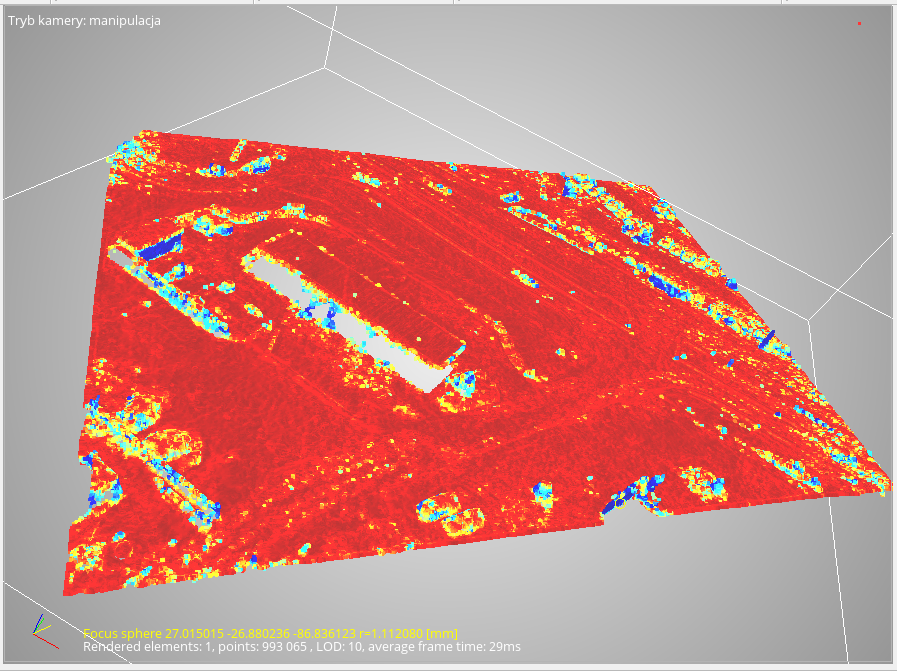
\includegraphics[width=0.85\textwidth]{smoothed_angles.png}
	\caption{Kąty między wektorami normalnymi punktów a osią Z - wygładzone}
	\label{fig:smoothedangles}
	\end{figure}
	
	Ostatnim krokiem jest segmentacja, która wykonywana jest w pętli for określoną ilość razy. Eksperymentalnie dobrana została wartość 10 iteracji. Daje ona zadowalające rezultaty i pozwala oszczędzić czas.\\
	\begin{figure}[h!]
		\centering
		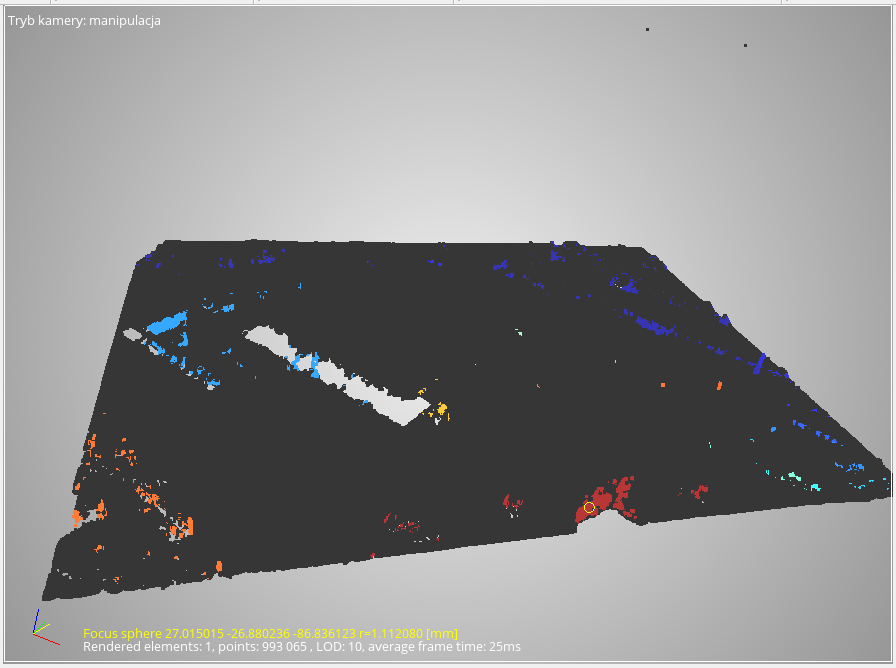
\includegraphics[width=0.85\textwidth]{wall_index.png}
		\caption{Ostateczny rezultat po segmentacji}
		\label{fig:after_segmentation}
	\end{figure}